\documentclass{article}
\usepackage{geometry}
 \geometry{
 a4paper,
 total={170mm,257mm},
 left=20mm,
 top=20mm,
 }

 \usepackage{caption}
\usepackage[export]{adjustbox} %% for picture frame
\usepackage[english]{babel}
\usepackage[utf8]{inputenc}
\usepackage{fancyhdr}

%%%question enviroment 

%%% Question Environment%%%  use 
%%% Question Environment%%%  use 
%%% Question Environment%%%  use \input{./QueENV.tex}   to include
%% Use \begin{Q}....\end{Q}

\newcounter{QC}
\setcounter{QC}{1}
\newenvironment{Q}[1]{
    \section{Question -\arabic{QC}} \stepcounter{QC}{\large\textbf{#1}}
}

%%% Question Environment%%%

   to include
%% Use \begin{Q}....\end{Q}

\newcounter{QC}
\setcounter{QC}{1}
\newenvironment{Q}[1]{
    \section{Question -\arabic{QC}} \stepcounter{QC}{\large\textbf{#1}}
}

%%% Question Environment%%%

   to include
%% Use \begin{Q}....\end{Q}

\newcounter{QC}
\setcounter{QC}{1}
\newenvironment{Q}[1]{
    \section{Question -\arabic{QC}} \stepcounter{QC}{\large\textbf{#1}}
}

%%% Question Environment%%%



\pagestyle{fancy}
\fancyhf{}
\rhead{\textit{LAB-2}}
\lhead{\textit{Pul074BEX004}}
\rfoot{\thepage}

%%% format and command for lab ans c and assembly

%%% Formating And Command for Embedded Lab   Assambly & C%%%


%%% Formatting And Command for Embedded Lab   Assembly & C%%%
%% 
%%% Formating And Command for Embedded Lab   Assambly & C%%%


%%% Formatting And Command for Embedded Lab   Assembly & C%%%
%% 
%%% Formating And Command for Embedded Lab   Assambly & C%%%


%%% Formatting And Command for Embedded Lab   Assembly & C%%%
%% \input{./asm c.tex}

%% \anscode{problem no. like 1,2,3...}{assembly code file }{ code file}


\usepackage{listings}
\usepackage{multicol}
\usepackage{mdframed}

\renewcommand{\lstlistlistingname}{List of Codes}
\renewcommand{\lstlistingname}{Code}


\setlength{\columnsep}{0.5cm}

\usepackage{xcolor}
\definecolor{codegreen}{rgb}{0,0.6,0}
\definecolor{codegray}{rgb}{0.4,0.4,0.4}
\definecolor{codepurple}{rgb}{0.58,0,0.82}
%\definecolor{backcolour}{rgb}{0.95,0.99,0.92}
\definecolor{backcolour}{rgb}{0,0,0}


\lstdefinestyle{customa}{
  backgroundcolor=\color{backcolour},   commentstyle=\color{codegreen},
  keywordstyle=\color{magenta},
  numberstyle=\tiny\color{codegray},
  stringstyle=\color{codepurple},
  basicstyle=\ttfamily\small\color{white},
  breakatwhitespace=false,
  breaklines=true,
  captionpos=b,
  morekeywords={MOV,ADD,ADDC,ACALL,INC,DJNZ,AJMP,RET,END,ORG,RR,JNC,SUBB,JC,DEC,ANL,SWAP,MUL,DIV,CLR,SETB},
  keepspaces=true,
  numbers=left,
  numbersep=5pt,
  showspaces=false,
  showstringspaces=false,
  showtabs=false,
  tabsize=4
}

\lstdefinestyle{customc}{
  backgroundcolor=\color{backcolour},   commentstyle=\color{codegreen},
  keywordstyle=\color{cyan},
  numberstyle=\tiny\color{codegray},
  stringstyle=\color{codepurple},
  basicstyle=\ttfamily\footnotesize\color{white},
  breakatwhitespace=false,
  breaklines=true,
  captionpos=b,
  keepspaces=true,
  language=C,
  numbers=left,
  numbersep=5pt,
  showspaces=false,
  showstringspaces=false,
  showtabs=false,
  tabsize=3
}




\newcommand {\anscode}[3]{

  \begin{center}
    \textbf{Assembly}
  \end{center}

  \begin{multicols}{2}
    \lstinputlisting[style=customa,nolol]{#2}
  \end{multicols}

  \begingroup
  \captionof{lstlisting}{Problem no. #1 Assembly}
  \endgroup


  \vspace{2 em}


  \begin{center}
    \textbf{C language }
  \end{center}
  \begin{multicols}{2}
    \lstinputlisting[style=customc,nolol]{#3}
  \end{multicols}

  \begingroup
  \captionof{lstlisting}{Problem no. #1 C language}
  \endgroup
}

%%% Formating And Command for Embedded Lab  Assambly & C%%%

%% \anscode{problem no. like 1,2,3...}{assembly code file }{ code file}


\usepackage{listings}
\usepackage{multicol}
\usepackage{mdframed}

\renewcommand{\lstlistlistingname}{List of Codes}
\renewcommand{\lstlistingname}{Code}


\setlength{\columnsep}{0.5cm}

\usepackage{xcolor}
\definecolor{codegreen}{rgb}{0,0.6,0}
\definecolor{codegray}{rgb}{0.4,0.4,0.4}
\definecolor{codepurple}{rgb}{0.58,0,0.82}
%\definecolor{backcolour}{rgb}{0.95,0.99,0.92}
\definecolor{backcolour}{rgb}{0,0,0}


\lstdefinestyle{customa}{
  backgroundcolor=\color{backcolour},   commentstyle=\color{codegreen},
  keywordstyle=\color{magenta},
  numberstyle=\tiny\color{codegray},
  stringstyle=\color{codepurple},
  basicstyle=\ttfamily\small\color{white},
  breakatwhitespace=false,
  breaklines=true,
  captionpos=b,
  morekeywords={MOV,ADD,ADDC,ACALL,INC,DJNZ,AJMP,RET,END,ORG,RR,JNC,SUBB,JC,DEC,ANL,SWAP,MUL,DIV,CLR,SETB},
  keepspaces=true,
  numbers=left,
  numbersep=5pt,
  showspaces=false,
  showstringspaces=false,
  showtabs=false,
  tabsize=4
}

\lstdefinestyle{customc}{
  backgroundcolor=\color{backcolour},   commentstyle=\color{codegreen},
  keywordstyle=\color{cyan},
  numberstyle=\tiny\color{codegray},
  stringstyle=\color{codepurple},
  basicstyle=\ttfamily\footnotesize\color{white},
  breakatwhitespace=false,
  breaklines=true,
  captionpos=b,
  keepspaces=true,
  language=C,
  numbers=left,
  numbersep=5pt,
  showspaces=false,
  showstringspaces=false,
  showtabs=false,
  tabsize=3
}




\newcommand {\anscode}[3]{

  \begin{center}
    \textbf{Assembly}
  \end{center}

  \begin{multicols}{2}
    \lstinputlisting[style=customa,nolol]{#2}
  \end{multicols}

  \begingroup
  \captionof{lstlisting}{Problem no. #1 Assembly}
  \endgroup


  \vspace{2 em}


  \begin{center}
    \textbf{C language }
  \end{center}
  \begin{multicols}{2}
    \lstinputlisting[style=customc,nolol]{#3}
  \end{multicols}

  \begingroup
  \captionof{lstlisting}{Problem no. #1 C language}
  \endgroup
}

%%% Formating And Command for Embedded Lab  Assambly & C%%%

%% \anscode{problem no. like 1,2,3...}{assembly code file }{ code file}


\usepackage{listings}
\usepackage{multicol}
\usepackage{mdframed}

\renewcommand{\lstlistlistingname}{List of Codes}
\renewcommand{\lstlistingname}{Code}


\setlength{\columnsep}{0.5cm}

\usepackage{xcolor}
\definecolor{codegreen}{rgb}{0,0.6,0}
\definecolor{codegray}{rgb}{0.4,0.4,0.4}
\definecolor{codepurple}{rgb}{0.58,0,0.82}
%\definecolor{backcolour}{rgb}{0.95,0.99,0.92}
\definecolor{backcolour}{rgb}{0,0,0}


\lstdefinestyle{customa}{
  backgroundcolor=\color{backcolour},   commentstyle=\color{codegreen},
  keywordstyle=\color{magenta},
  numberstyle=\tiny\color{codegray},
  stringstyle=\color{codepurple},
  basicstyle=\ttfamily\small\color{white},
  breakatwhitespace=false,
  breaklines=true,
  captionpos=b,
  morekeywords={MOV,ADD,ADDC,ACALL,INC,DJNZ,AJMP,RET,END,ORG,RR,JNC,SUBB,JC,DEC,ANL,SWAP,MUL,DIV,CLR,SETB},
  keepspaces=true,
  numbers=left,
  numbersep=5pt,
  showspaces=false,
  showstringspaces=false,
  showtabs=false,
  tabsize=4
}

\lstdefinestyle{customc}{
  backgroundcolor=\color{backcolour},   commentstyle=\color{codegreen},
  keywordstyle=\color{cyan},
  numberstyle=\tiny\color{codegray},
  stringstyle=\color{codepurple},
  basicstyle=\ttfamily\footnotesize\color{white},
  breakatwhitespace=false,
  breaklines=true,
  captionpos=b,
  keepspaces=true,
  language=C,
  numbers=left,
  numbersep=5pt,
  showspaces=false,
  showstringspaces=false,
  showtabs=false,
  tabsize=3
}




\newcommand {\anscode}[3]{

  \begin{center}
    \textbf{Assembly}
  \end{center}

  \begin{multicols}{2}
    \lstinputlisting[style=customa,nolol]{#2}
  \end{multicols}

  \begingroup
  \captionof{lstlisting}{Problem no. #1 Assembly}
  \endgroup


  \vspace{2 em}


  \begin{center}
    \textbf{C language }
  \end{center}
  \begin{multicols}{2}
    \lstinputlisting[style=customc,nolol]{#3}
  \end{multicols}

  \begingroup
  \captionof{lstlisting}{Problem no. #1 C language}
  \endgroup
}

%%% Formating And Command for Embedded Lab  Assambly & C%%%
%%%%>>>>>>>........
%%%%%% include  Titles.%%%% use \input{./CP}%%%
%%%use """"""""    \CP{}{}{}{}   """" %%%% and 4 argument to craete Title page 
%%%%%%%%%%%%%%%%%%%%%%%%%%%%%%%%%%%%%%%%%%%%%%%%%%%%%%%%%%%%%%%%%
%%%argument number
%% 1=major header ## Course name 
%% 2=minor4 heading ## lab/assignmet no
%% 3=Title  ## Assignment or Lab title
%% 4=submitted to::## input receiver Name"
%%%%%%%%%%%%%%%%%%%%%%%%%%%%%%%%%%%%%%%%%%%%%%%%%%%%%%%%%%%%%%%%%


\usepackage{mathpazo} % Palatino font
\usepackage{graphicx}
\usepackage{float}

%%% format and command for lab ans c and assembly

\newcommand{\HRule}{\rule{\linewidth}{0.4mm}} % Defines a new command for horizontal lines, change thickness here



%----------------------------------------------------------------------------------------
%	TITLE PAGE
%----------------------------------------------------------------------------------------


\newcommand{\CP}[4]{ \begin{titlepage} % Suppresses displaying the page number on the title page and the subsequent page counts as page 1
		%%%%  univerdity logo%%
		\begin{figure}[H]
			\centering
			
\includegraphics[scale=0.13]{tulogo.jpg}
		\end{figure}
		%%% end university logo

		\center % Centre everything on the page

		%------------------------------------------------
		%	Headings
		%------------------------------------------------

		\textsc{\huge Institute of Engineering \\ Central Campus,Pulchowk}\\[1.5cm] % Main heading such as the name of your university/college

		\textsc{\Large #1}\\[0.5cm] % Major heading such as course name

		\textsc{\large #2}\\[0.5cm] % Minor heading such as assignment no./ lab no.

		%------------------------------------------------
		%	Title
		%------------------------------------------------

		\HRule\\[0.4cm]

		{\Huge\bfseries #3}\\[0.4cm] % Title of your document

		\HRule\\[1.5cm]

		%------------------------------------------------
		%	Author(s)
		%------------------------------------------------
		\vfill\vfill
		\begin{minipage}{0.4\textwidth}
			\begin{flushleft}
				\large{
				\textbf{Submitted BY:}\\
				{\normalsize AMRIT PRASAD PHUYAL}\\ % NAME
				{\normalsize Roll: PULL074BEX004}} % Roll
			\end{flushleft}
		\end{minipage}
		~
		\begin{minipage}{0.4\textwidth}
			\begin{flushright}
				\large
				\textbf{Submitted To:}\\
				{ \normalsize{#4}\\ }% recepent's  Name 
				{\normalsize Department of Electronics and Computer Engineering}
			\end{flushright}
		\end{minipage}

		%------------------------------------------------
		%	Date
		%------------------------------------------------

		\vfill\vfill\vfill % Position the date 3/4 down the remaining page

		{\large\today} % Date, change the \today to a set date if you want to be precise

		\vfill % Push the date up 1/4 of the remaining page

	\end{titlepage}
}

\begin{document}

%----------------------------------------------------------------------------------------
%	TITLE PAGE
%----------------------------------------------------------------------------------------
\CP{Embedded system}{LAB \#2}
{Interfacing 7-Segment LED Display with 8051/8052 Micro-controller}
{Department of Electronics and Computer Engineering}




%----------------------------------------------------------------------------------------
\pagenumbering{gobble}
\tableofcontents
\pagebreak
\listoffigures
\pagebreak
\lstlistoflistings
\pagebreak
\pagenumbering{arabic}
\section{Introduction}
\subsection{Microcontroller}

A microcontroller is an integrated circuit ( IC), usually via an MPU, memory and certain peripherals, to control other parts of an electronic system .
These devices are optimized for embed-in applications that require agile and agile processing, digital, analog or electromechanical interactions.
\subsection{8051 Microcontroller}
In 1981, Intel introduced an 8-bit microcontroller called the 8051. It was referred as system on a chip because it had 128 bytes of RAM, 4K byte of on-chip ROM,
two timers, one serial port, and 4 ports (8-bit wide), all on a single chip.\\\\
The different features of the 8051 microcontroller include:
\begin{itemize}
    \item 4KB bytes on-chip program memory (ROM)
    \item 128 bytes on-chip data memory (RAM)
    \item Four register banks
    \item 128 user defined software flags
    \item 8-bit bidirectional data bus
    \item 16-bit unidirectional address bus
    \item 32 general purpose registers each of 8-bit
    \item 16 bit Timers (usually 2, but may have more or less)
    \item Three internal and two external Interrupts
    \item Four 8-bit ports,(short model have two 8-bit ports)
    \item 16-bit program counter and data pointer
    \item 8051 may also have a number of special features such as UARTs, ADC, Op-amp, etc.
\end{itemize}
\begin{figure}[H]
    \centering
    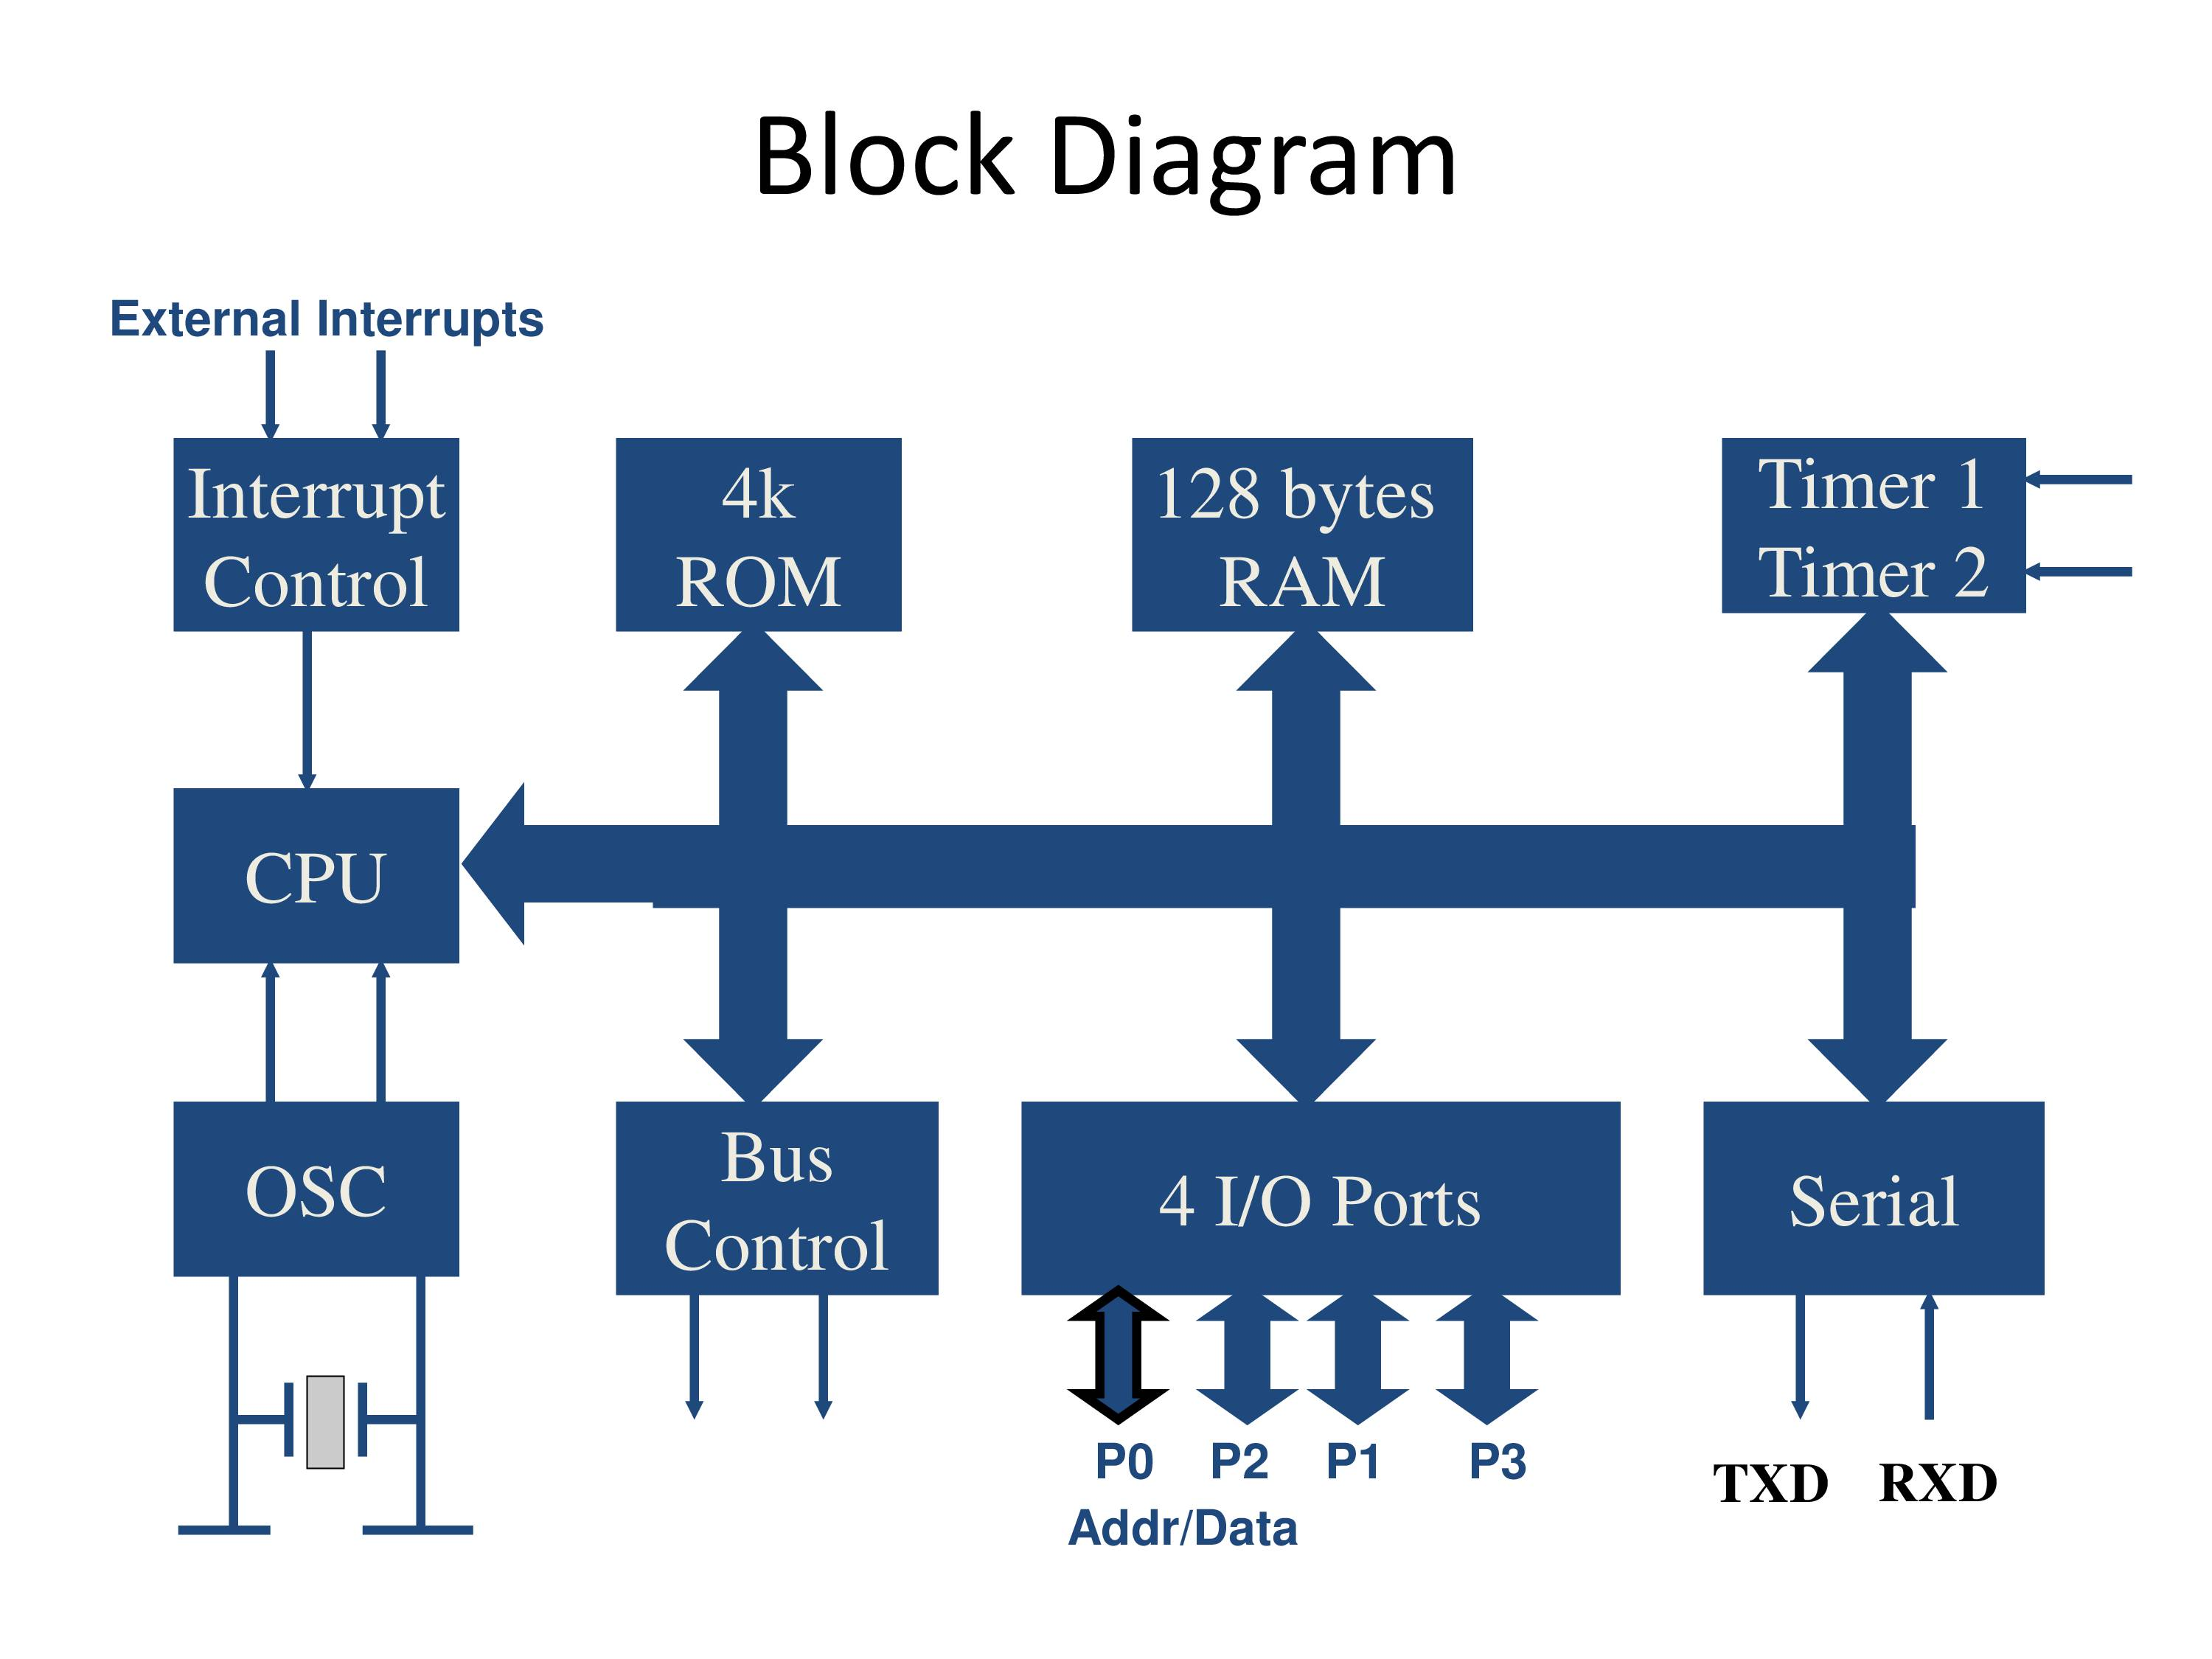
\includegraphics[scale=0.52,cframe=blue 0.5pt 3pt]{./block_diagram.jpg}
    \textit{\caption{Block diagram of 8051 microcontroller}}

\end{figure}

\subsection{7-Segment LED Display}
A seven segment display module is an electronic device used to display digital numbers and
it is made up of seven LED segments. LEDs are PN-junction diodes which emit energy by a process called electroluminescence.
Because of the small size of the LEDs, it is really easy for a number of them to be connected together to make a unit like seven segment display.
The light energy is emitted as ‘photons’ when it is forward biased by a voltage applied across its junctions.
In a seven segment display module, seven LED s are arranged in a rectangle. Sometimes,
an additional LED is seen in a seven segment display unit which is meant for displaying a decimal point.

Features of seven segment Display:-

\begin{itemize}
    \item Available in two modes Common Cathode (CC) and Common Anode (CA)
    \item Available in many different sizes like 9.14mm,14.20mm,20.40mm,38.10mm,57.0mm and 100mm (Commonly used/available size is 14.20mm)
    \item Available colours: White, Blue, Red, Yellow and Green (Res is commonly used)
    \item Low current operation
    \item Better, brighter and larger display than conventional LCD displays.
    \item Current consumption : 30mA / segment
    \item Peak current : 70mA
\end{itemize}

The displays common pin is generally used to identify which type of 7-segment display it is. As each LED has two connecting pins,
one called the “Anode” and the other called the “Cathode”, there are therefore two types of LED 7-segment display called: Common Cathode (CC) and Common Anode (CA).
The difference between the two displays, as their name suggests,
is that the common cathode has all the cathodes of the 7-segments connected directly together and the common anode has all the anodes of the 7-segments connected together
\begin{figure}[H]
    \centering
    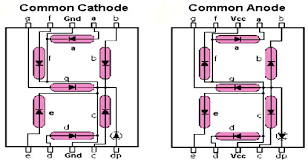
\includegraphics[scale=1.1,cframe=blue 0.5pt 3pt]{./Common cathode vs common anode.png}
    \textit{\caption{Common cathode vs Common anode 7 segment display}}
\end{figure}


\begin{figure}[H]
    \centering
    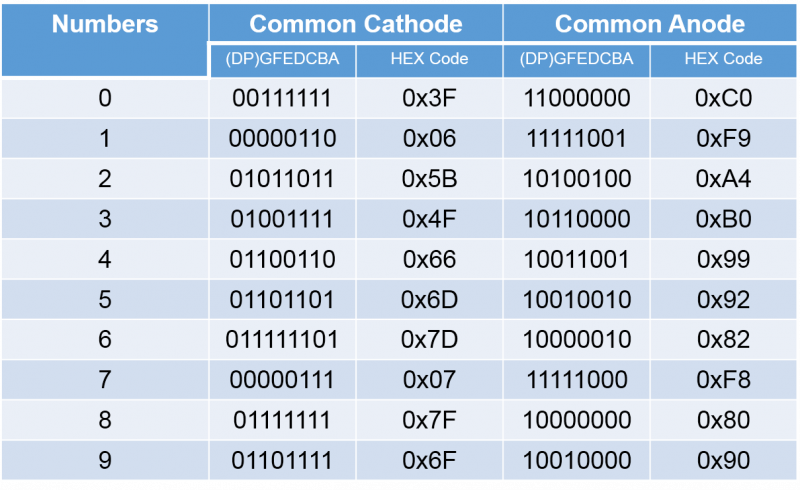
\includegraphics[scale=0.65,cframe=blue 0.5pt 3pt]{./Dispaly codes.png}
    \textit{\caption{Lookup table for Common anode and Common Cathode}}
\end{figure}

\subsection{Applications}
\begin{itemize}
    \item Used in applications where font size is required to be bigger
    \item Microcontroller Independent, hence used in small circuit projects
    \item Used in combination with four segments to display measurement/sensor value  with four characters
    \item Has bright illumination, hence used where display are required to work in low light or dark conditions
\end{itemize}


\end{document}